\documentclass[12pt]{article}
%\usepackage[english]{babel}
\RequirePackage[spanish]{babel}
\usepackage[spanish]{babel}
\usepackage{graphicx}
%\usepackage[pdftex,bookmarks,colorlinks,breaklinks]{hyperref}  % PDF hyperlinks, with coloured links
%\usepackage[spanish]{babel}
\usepackage[pdftex,bookmarks,breaklinks]{hyperref}  % PDF hyperlinks, with coloured links
%\usepackage[spanish]{babel}
\usepackage[utf8]{inputenc}
\usepackage{enumerate}
\usepackage{longtable}
\usepackage{subfig}
\usepackage{epstopdf}
\usepackage{fullpage}
\usepackage{url}
\usepackage{colortbl}
\usepackage{lscape}
\usepackage{float}
\renewcommand{\baselinestretch}{1.5}
\usepackage{multirow}
\parskip 3ex % espacio entre parrafos.
\makeatletter
\renewcommand\paragraph{\@startsection{paragraph}{4}{\z@}%
	{-2.5ex\@plus -1ex \@minus -.25ex}%
	{1.25ex \@plus .25ex}%
	{\normalfont\normalsize\bfseries}}
\makeatother
\setcounter{secnumdepth}{4} % how many sectioning levels to assign numbers to
\setcounter{tocdepth}{4}    % how many sectioning levels to show in ToC

\begin{document}
%%%%%%%%%%%%%%% PORTADA %%%%%%%%%%%%%%%%%%
\pagestyle{empty}
\begin{figure}
   \centering
   
\includegraphics[scale=.5]{imgs/logo_utal.png}
\end{figure}

\begin{center}
Facultad de Ingeniería\\
Escuela de Ingeniería en Bioinformática\\
Ingeniería de Software\\
\bigskip\bigskip\bigskip\bigskip

\rule{14cm}{0.5mm}

\begin{Huge}\textbf{ Proyecto Juego Espacios Turísticos en 360°}\end{Huge}

\rule{14cm}{0.5mm}

\bigskip\bigskip\bigskip\bigskip
\bigskip\bigskip\bigskip\bigskip
\bigskip\bigskip\bigskip\bigskip
%\bigskip\bigskip\bigskip\bigskip
%\bigskip\bigskip\bigskip\bigskip

\begin{tabular*}{14cm}{l@{\extracolsep{\fill}}r}
\textbf{\emph{Integrantes:}} & \textbf{\emph{Profesor:}}\\
Felipe Durán & Felipe Besoain\\
Ignacio Gajardo & \textbf{\emph{Ayudante:}}\\
Alex Molina & José Francisco Riffo\\
\end{tabular*}
\end{center}

%%%%%%%%%%%%%%%%%%%%%%%%%%%%%%%%%%%%%%%
\newpage
\pagestyle{plain}
\tableofcontents

%%%%%%%%%%%%%%%%%%%%%%%%%%%%%%%%%%%%%%%
\newpage
\listoffigures 

%%%%%%%%%%%%%%%%%%%%%%%%%%%%%%%%%%%%%%%
\newpage
\listoftables


%%%%%%% INTRODUCCIÓN %%%%%%%%%%%%%%%%
\newpage
\section{Introducción}
\subsection{Propósito}
Este documento se muestra el modelo de trabajo utilizado para la creación de una aplicación con fines de entretener a su usuario fomentando sus habilidades creativas. Si bien la información encontrada requiere un mínimo conocimiento de programación básica y de base de datos, su nivel de entrada es bajo. Tomando en cuenta su propósito se recomienda a sus lectores tener un interés en lo que refiere a la creación de aplicaciones móviles para un grupo de usuarios casuales. Como lo muestra su índice, la estructura de este informe se basará en las tres áreas principales del desarrollo de aplicaciones, estas siendo programación, diseño y material audiovisual.
\subsection{Descripción breve del problema}
En base a la información entregada en el documento base para el desarrollo de la aplicación se encontraron 3 factores principales para una realización correcta del proyecto. 

El primero es la realización de una base de datos, que cuenta como la parte central para la creación de esa aplicación. Para esta área se contará con el conocimiento del equipo de programación para llegar a una conclusión de como implementarla, ya sea con el uso de aplicaciones externas o no.

 El segundo siendo el diseño de la aplicación ya que solo se entregó una simple descripción de actividades básicas que requiere el software, lo que, aunque entrega una libertad al equipo desarrollador también le pide mas trabajo en los aspectos más detallados de este. Para solucionar esta situación se le dará un enfoque en la preproducción del proyecto solo para llegar a una idea mas desarrollada del producto final.
 
Finalmente, el tercero es el material audiovisual necesario para la creación del software con la necesidad de usar imágenes en 360. Tomando en cuenta que el equipo de desarrollo se encuentra en ciudades distintas y la situación mundial se tendrá que recurrir a la búsqueda de este material por internet, asegurándose de que este se encuentre disponible para su uso público.


%%%%%%% PLANIFICACIÓN DE TRABAJO %%%%%%%%%%%%
\newpage
\section{Planificación del Trabajo}

\subsection{Descripción del grupo de trabajo}
A continuación se especificará el grupo de trabajo, el cual estará encargado del desarollo de la aplicación de conquista de espacios turísticos en 360°. Se especificará su ID, nombre, conocimientos, rol y contacto de cada uno de los integrantes del grupo de trabajo.

\begin{table}[H]
    \centering
        \begin{tabular}{|l | p{12cm} |}        
        \hline
        \textbf{ID} & FD \\
        \hline
        \textbf{Nombre} & Felipe Durán \\
        \hline
        \textbf{Conocimientos} & Experiencia en lenguaje de programación como Phython, C, C++, C\# , Java, JavaScript, Kotlin y Conocimientos con base de datos MySQL. \\
        \hline
        \textbf{Rol} & Planificador y Programador de la aplicación movil. \\    
        \hline
        \textbf{Contacto} & fduran16@alumnos.utalca.cl \\
        \hline            
        \end{tabular}
    \caption{Descripción Personal FD}
\end{table}


\begin{table}[H]
    \centering
        \begin{tabular}{|l | p{12cm} |}        
        \hline
        \textbf{ID} & IG \\
        \hline
        \textbf{Nombre} & Ignacio Gajardo \\
        \hline
        \textbf{Conocimientos} & Experiencia en lenguaje de programación como Phython, C, C++, C\# , Java, JavaScript, Kotlin y Conocimientos con base de datos MySQL. \\
        \hline
        \textbf{Rol} & Planificador y Programador de la aplicación movil. \\    
        \hline
        \textbf{Contacto} & igajardo16@alumnos.utalca.cl \\
        \hline            
        \end{tabular}
    \caption{Descripción Personal IG}
\end{table}


\begin{table}[H]
    \centering
        \begin{tabular}{|l | p{12cm} |}        
        \hline
        \textbf{ID} & AM \\
        \hline
        \textbf{Nombre} & Alex Molina \\
        \hline
        \textbf{Conocimientos} & Experiencia en lenguaje de programación como Phython, C, C++, C\# , Java y Conocimientos con base de datos MySQL. \\
        \hline
        \textbf{Rol} & Planificador y Programador de la aplicación movil. \\    
        \hline
        \textbf{Contacto} & amolina16@alumnos.utalca.cl \\
        \hline            
        \end{tabular}
    \caption{Descripción Personal AM}
\end{table}

Los recursos que se utilizarán en el desarrollo del proyecto del software de conquista de espacios turísticos en 360° son:

\begin{table}[H]
    \centering
        \begin{tabular}{|l | p{12cm} |}        
        \hline
        \textbf{ID} & FD\_Notebook \\
        \hline
        \textbf{Tipo de dispositvo} & Notebook \\
        \hline
        \textbf{Sistema operativo} & Window 10 Home \\
        \hline
        \textbf{Modelo} & Asus \\
        \hline
        \textbf{Procesador} & AMD FX-9830P RADEON R7 \\    
        \hline            
        \end{tabular}
    \caption{Recurso FD\_Notebook}
\end{table}


\begin{table}[H]
    \centering
        \begin{tabular}{|l | p{12cm} |}        
        \hline
        \textbf{ID} & IG\_Notebook \\
        \hline
        \textbf{Tipo de dispositvo} & Notebook \\
        \hline
        \textbf{Sistema operativo} & Window 10 Home \\
        \hline
        \textbf{Modelo} & MSI \\
        \hline
        \textbf{Procesador} & Intel Core i7-6700 \\    
        \hline            
        \end{tabular}
    \caption{Recurso IG\_Notebook}
\end{table}

\begin{table}[H]
    \centering
        \begin{tabular}{|l | p{12cm} |}        
        \hline
        \textbf{ID} & AM\_Notebook \\
        \hline
        \textbf{Tipo de dispositvo} & Notebook \\
        \hline
        \textbf{Sistema operativo} & Window 10 Home \\
        \hline
        \textbf{Modelo} & HP \\
        \hline
        \textbf{Procesador} & Intel Core i5-7300 \\    
        \hline            
        \end{tabular}
    \caption{Recurso AM\_Notebook}
\end{table}

\subsection{Estimación de esfuerzo}
Se a realizado un análisis de todos los aspectos posibles que serán parte del desarrollo del software y que competen a la estimación de esfuerzo. Sin embargo, todo lo analizado queda sujeto a modificaciones, debido principalmente a que el proyecto está aún en desarrollo y no se encuentra una versión base o una visión profesionalmente detallada de las iteraciones para desarrollar el producto final. Tanto a nivel de programación como de diseño a de ser necesaria una frecuente revisión y actualización con cada iteración y avance en este proyecto.

Según lo conversado, pactado y analizado con el equipo de desarrollo en la primera iteración, el análisis del proyecto se puede apreciar en las siguientes graficas de estimación de puntos de esfuerzo.

\begin{figure}[H]
	\centering
	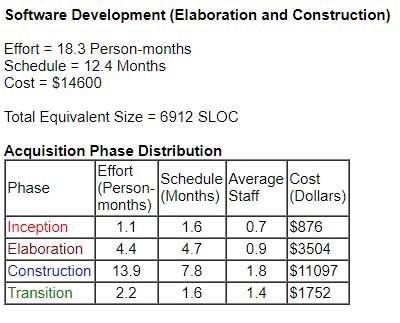
\includegraphics[width=16cm, height=9cm]{imgs/1.JPG}
	\caption{Precio de mese hombre}
\end{figure}

\begin{figure}[H]
	\centering
	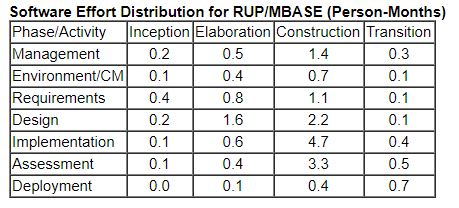
\includegraphics[scale=1.7]{imgs/2.JPG}
	\caption{Tabla Mes-hombre}
\end{figure}

\begin{figure}[H]
	\centering
	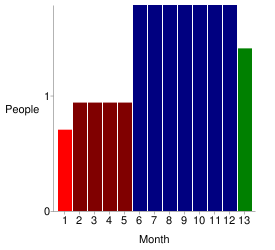
\includegraphics[width=16cm, height=9cm]{imgs/Grafica.png}
	\caption{Grafica Mes-hombre}
\end{figure}

\begin{figure}[H]
	\centering
	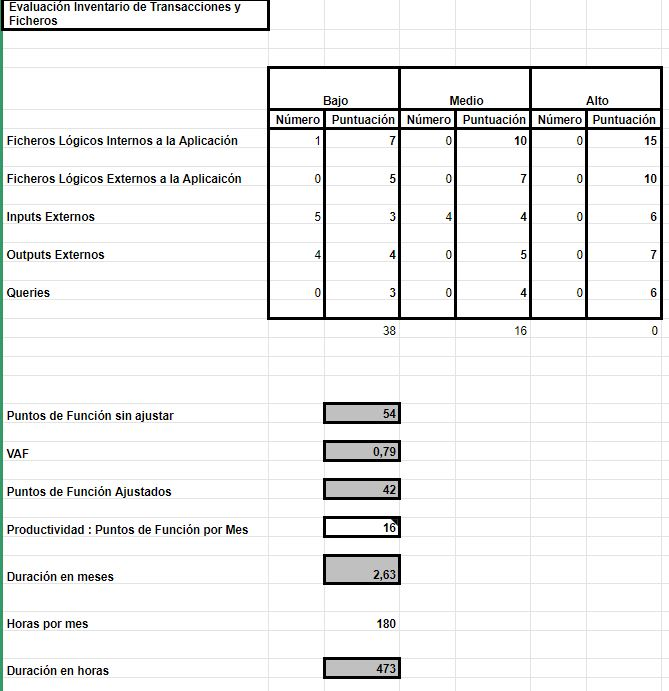
\includegraphics[width=16cm, height=9cm]{imgs/Estimacion de PF.JPG}
	\caption{Estimacion de puntos de esfuerzo}
\end{figure}

\subsection{Asignación de recursos}
En esta parte va la carta gantt
"Estamos arreglando esta parte"

\begin{table}[H]
    \begin{center}
        \begin{tabular}{| m{6cm} | m{3cm} | m{2cm} | m{4cm} |}        
        	\hline 
        	Tarea & Categorìa & Prioridad & Asignado a\\
        	\hline
        	Dependencias & Implementación & Medio & Alex Molina\\
        	\hline
        	Modelo de Implantación & Implementación & Medio & Ignacio Gajardo\\
        	\hline
        	Codigo Fuente & Implementación & Medio & Felipe Duran\\
        	\hline
        \end{tabular}
    \caption{Asignacion del personal a sus distintos cargos}
    \end{center}
\end{table}
\subsection{Planificación temporal de actividades}
\textbf{Gráficos de la planificación actual:}

\begin{figure}[H]
 \centering
  \subfloat[prioridad]{
   \label{f:gato}
    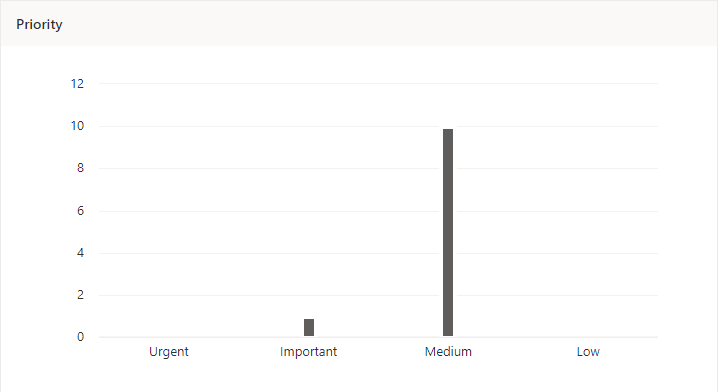
\includegraphics[width=7cm, height=8cm]{imgs/planner_priority.png}}
  \subfloat[Gráfico de barra]{
   \label{f:tigre}
    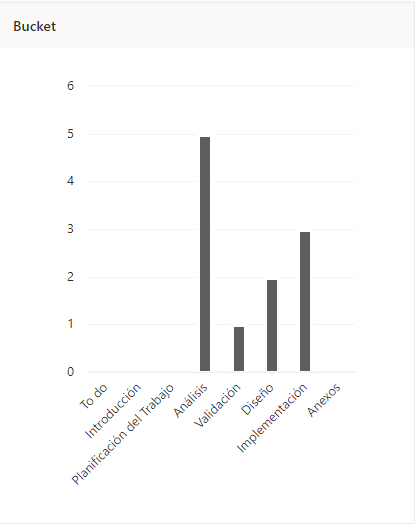
\includegraphics[width=7cm, height=8cm]{imgs/planner_bucket.png}}
 \caption{Estado de la planificación}
 \label{f:Graficos}
\end{figure}

%%%%%%%%%% ANALISIS %%%%%%%%%%%%%%
\newpage
\section{Análisis}

\subsection{Contexto}
\subsubsection{Descripción General}
Como todo proyecto el paso inicial es un análisis del objetivo a realizar, y este caso no es la excepción. La información utilizada para este análisis consistió en una explicación concisa de los requerimientos necesarios de la aplicación, principalmente mecánicas y características que debe contener la versión final, la cual concluyó que su desarrollo debe tener un énfasis en el funcionamiento básico de esta.\\
El resultado del análisis llevó a una descripción propia del proyecto, el resultado final es una aplicación que funcione como herramienta interactiva basada en una enseñanza de exploración y el contenido que esta acción entrega. La parte lúdica del aprendizaje se ve con la implementación de un sistema inspirado en juegos de mesa donde un numero plural de usuarios toman turnos para realizar acciones y avanzar en un mapa para llegar a una meta final. Cada turno se les entrega a los jugadores una imagen en 360 grados de un área o paisaje en particular y una cantidad de conceptos escogidos al azar (estas palabras son encontradas en una base de datos) con esto los usuarios tendrán que concebir una historia usando los datos mencionados. Al final todos tendrán que votar por otro usuario que consideren haber creado la mejor historia, el usuario ganador avanza un espacio y se sigue la misma idea cada turno hasta que uno llegue al final.
En cuanto a los problemas mencionados en el punto 1.1.2 se tomó la esquematización de estos y se analizaron con profundidad. La base de datos a utilizar debe centrarse en una cantidad reducida de usuarios (cuantos jugadores simultáneos se encuentran), también se llegó a la conclusión de que cada usuario cuenta con su propio dispositivo (un smartphone) por lo que se requerirá uso de internet para facilitar los datos a los usuarios. El análisis del proyecto y de la situación del equipo de desarrollo encuentra que el uso de Android studio (con el lenguaje de kotlin) y la implementación de firebase a este es la opción mas viable.\\
El diseño de la aplicación lleva a la conclusión de comenzar la estructura principal de este (encontrado en el caso de estudio entregado al equipo) dándole una mayór importancia la implementación las mecánicas claves recibidas, asegurándose de que estas funcionen sin problemas antes de ampliar o expandir el desarrollo del proyecto.
Lo que respecta a material audiovisual el equipo encarga en las ultimas fases de desarrollo un tiempo en particular para la búsqueda e implementación de sonidos o imágenes necesarias, y al igual que los otros casos, dándole mayor importancia a las direcciones entregadas al equipo, en este caso siendo el uso de imágenes en 360 grados en la aplicación.

\subsubsection{Descripción de Clientes y Usuarios:}
Luego de un análisis realizado en base a la información entregada del resultado esperado por la aplicación se a encontrado un perfil definido para tanto clientes como usuarios.
Los clientes fueron concretados en un grupo centrado en una o más de las mecánicas principales presentadas. En específico, la vista de paisajes y lugares geográficos en 360 grados le interesa a un grupo enfocado en turismo como forma de enseñar los paisajes de una zona o región en particular. El otro enfoque encontrado en la aplicación que puede llamar la atención para un cliente es la mecánica de crear historias en base a palabras encontradas en una base de datos, tomando con mayor atención la parte literaria de juego centrada en la creatividad del usuario, pero siendo usada como forma de enseñanza.
Por otro lado, durante el desarrollo de la aplicación los usuarios tomaron un enfoque más genérico que el de los clientes, se encontró que en cualquier caso estos tenían requerimientos  simples ya que lo más importante es facilitarles el uso de esta. El usuario objetivo se identificó como un individuo o individua con un conocimiento basico de tecnologia, tomando en cuenta de que la plataforma utilizada es de smartphones, que entienda el concepto de identificarse de forma virtual con su correo electronico ademas de entender las reglas básicas del juego. Además, este debe tener un conocimiento literario de enseñanza básica como mínimo, tomando en cuenta de que el “input” principal de parte del usuario es crear y contar una historia en base a un grupo de palabras entregadas.
\subsection{Especificación de Requerimientos}
\subsubsection{Funciones del Sistema}
Funciones evidentes:
\\	-Registrar nuevo usuario.
\\	-Realizar autentificacion con correo.
\\	-Realizar autentificacion con contraseña.
\\	-Realizar autentificacion con Gmail.
\\	-Mostrar imagenes en 360°.
\\	-Sistema de turnos.
\\	-Generar lista de palabras.
\\	-Multijugador global.\\\\
Funciones ocultas:
\\	-Cargar imagenes en 360°.
\\	-Crear base de datos para palabras.
\\	-Crear base de datos para puntajes.\\\\
Funciones Suérfluas:
\\	-Generar una tabla de puntajes.
\subsubsection{Atributos del Sistema}
-Intuitiva: Debe ser de facil entendimiento para el usuario final, es decir, el ususario debe saber que hacer o como empezar a jugar sin mucha complejidad\\
-Optimizado: La aplicación debe usar recursos del celular solo de ser sumamente necesario\\
-Baja frecuencia de fallos: El Programa no debe presentar mas de cuatro fallos al mes\\
-Facilidad de configuración: Debe ser sencillo para el usuario customizar a su gusto la aplicacion\\
-Facilidad de mantenimiento: A los programadores y gente encargada de mantener la aplicacion dfuncionando se les debe hacer sencillo ingresar al codigo, entenderlo y aplicar las reparaciones\\
\subsubsection{Atributos por Función}
\begin{table}[H]
    \begin{center}
        \begin{tabular}{| l | m{6cm} | m{6cm} |}        
        	\hline 
        	Ref\# & Función & Categoria\\
        	\hline
        	... & ... & ...\\
        	\hline
        	... & ... & ...\\
        	\hline
        	... & ... & ...\\
        	\hline
        \end{tabular}
    \caption{Funciones agrupadas}
    \end{center}
\end{table}
\newpage
\subsection{Actores}
Jugador : La aplicación está hecha para que sea utilizada por usuarios, su último fin es entretener a un público y es quien debiera ser su actor final y principal.\\
2. Escaner QR: Se utiliza para escanear la imagen en 360°.\\
3. FireBase : Permite el contacto entre la aplicación y múltiples herramientas como lo son la base de datos, el guardado de respaldo, etc. Además hace nexo entre la aplicación y los siguientes actores:\\
a. -Base de Datos : La aplicación debe mantener contacto con la base de datos de forma directa, para poder acceder a las palabras, imágenes, usuarios, etc.\\
b. -Gmail : Herramienta principal para identificar al usuario por medio de correo electrónico.
\subsection{Casos de Uso}
\begin{table}[H]
    \begin{center}
        \begin{tabular}{| l | m{12cm} |}        
        	\hline 
        	Identificador & 1\\
        	\hline
        	Caso de Uso & Jugar una partida de Conquista Turística
360°\\
        	\hline
        	Tipo & Primario\\
        	\hline
        	Descripción & El programa le muestra al jugador 4 palabras por pantalla, el jugador las ve y las usa para crear una historia. Los demás jugadores votan por la creatividad de la historia en la applicacion y deciden que el jugador puede avanzar, el programa recibe el feedback de los jugadores por pantalla y mueve al jugador a la siguiente posición.\\
        	\hline
        \end{tabular}
    \caption{Primer caso de uso}
    \end{center}
\end{table}

\begin{table}[H]
    \begin{center}
        \begin{tabular}{| l | m{12cm} |}        
        	\hline 
        	Identificador & 2\\
        	\hline
        	Caso de Uso & Iniciar sesión\\
        	\hline
        	Tipo & Primario\\
        	\hline
        	Descripción & ...\\
        	\hline
        \end{tabular}
    \caption{Segundo caso de uso}
    \end{center}
\end{table}

\begin{table}[H]
    \begin{center}
        \begin{tabular}{| l | m{12cm} |}        
        	\hline 
        	Identificador & 3\\
        	\hline
        	Caso de Uso & Generar lista de palabras\\
        	\hline
        	Tipo & Primario\\
        	\hline
        	Descripción & ...\\
        	\hline
        \end{tabular}
    \caption{Tercer caso de uso}
    \end{center}
\end{table}

\begin{table}[H]
    \begin{center}
        \begin{tabular}{| l | m{12cm} |}        
        	\hline 
        	Identificador & 4\\
        	\hline
        	Caso de Uso & Iniciar sesión\\
        	\hline
        	Tipo & Primario\\
        	\hline
        	Descripción &...\\
        	\hline
        \end{tabular}
    \caption{Cuarto caso de uso}
    \end{center}
\end{table}

\begin{table}[H]
    \begin{center}
        \begin{tabular}{| l | m{12cm} |}        
        	\hline 
        	Identificador & 5\\
        	\hline
        	Caso de Uso & Calificar jugadores\\
        	\hline
        	Tipo & Primario\\
        	\hline
        	Descripción & ...\\
        	\hline
        \end{tabular}
    \caption{Quinto caso de uso}
    \end{center}
\end{table}
\subsubsection{Caso de Uso Esencial}
\subsubsection{Diagrama de Caso de Uso}
\subsubsection{Contrato}
\subsubsection{Modelo Conceptual}
\subsubsection{Diagrama de Secuencia o Colaboración}
\subsubsection{Priorización}

\subsection{Modelo de Dominio}
\subsubsection{Entidades Reconocidas}
\subsubsection{Modelo de Dominio}
\subsubsection{Matriz de Rastreabilidad}

%%%%%%%%% VALIDACION %%%%%%%%%%%
\newpage
\section{Validación}
 Las motivaciones del empleador han sido comprendidas y se han tomado las consideraciones requeridas para responder a su motivación, para esto se han aplicado funciones como iniciar secion con alguna cuenta, poder visualizar inamegenes en 360° de lugares turisticos, caracteristicos o iconicos de la regien del maule, presentar un diseño que sea relajante, entre otras funciones mencionadas con anterioridad en este documento.
\subsection{Prototipo de validación funcional}
A continuación se presentan algunas capturas de pantalla obtenidas de la aplicación para mostrar el progreso y el diseño realizado por los desarrolladores.
\begin{figure}[H]
	\centering
	\subfloat[Screenshot de la app N°01]
	{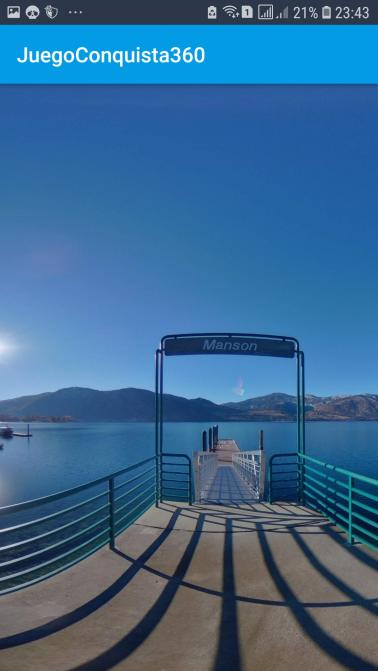
\includegraphics[width=5cm, height=8cm]{imgs/Screenshot1.jpg}}
	\subfloat[Screenshot de la app N°02]
	{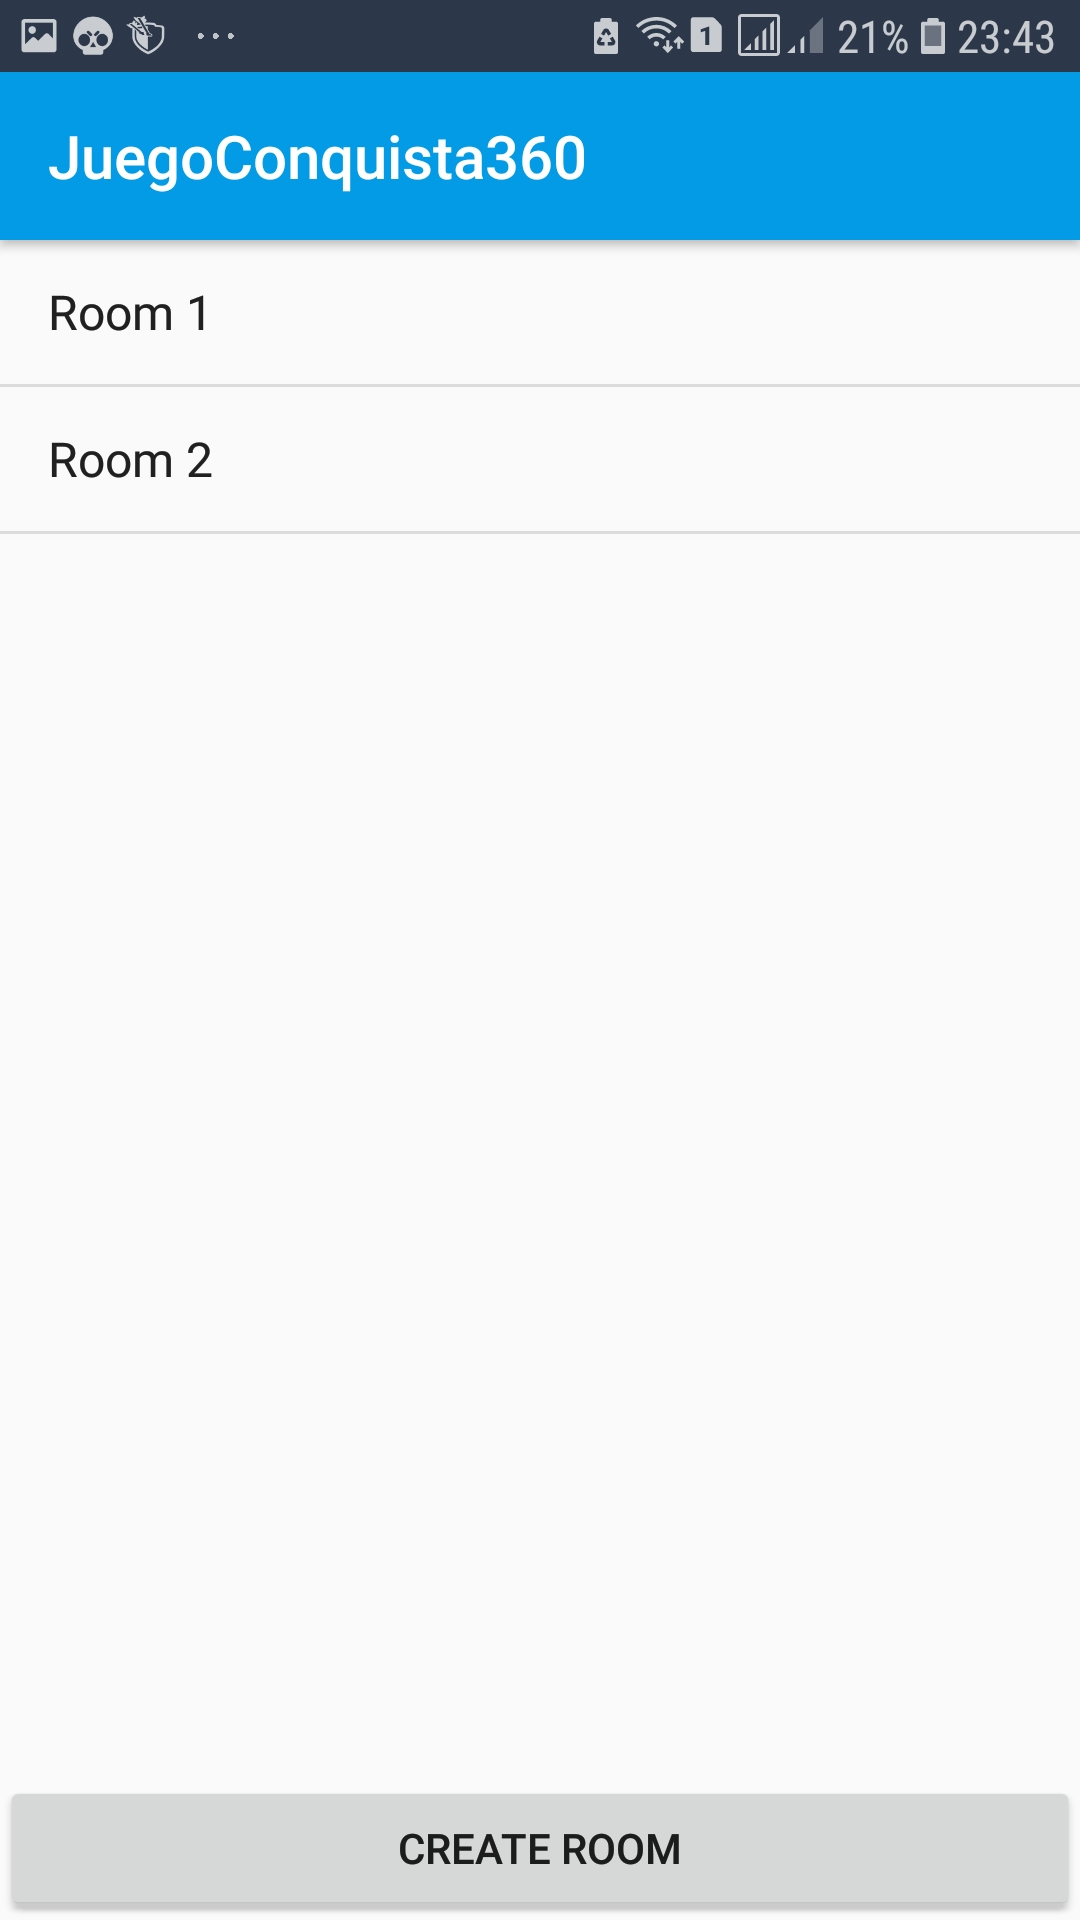
\includegraphics[width=5cm, height=8cm]{imgs/Screenshot2.jpg}}
	\subfloat[Screenshot de la app N°03]
	{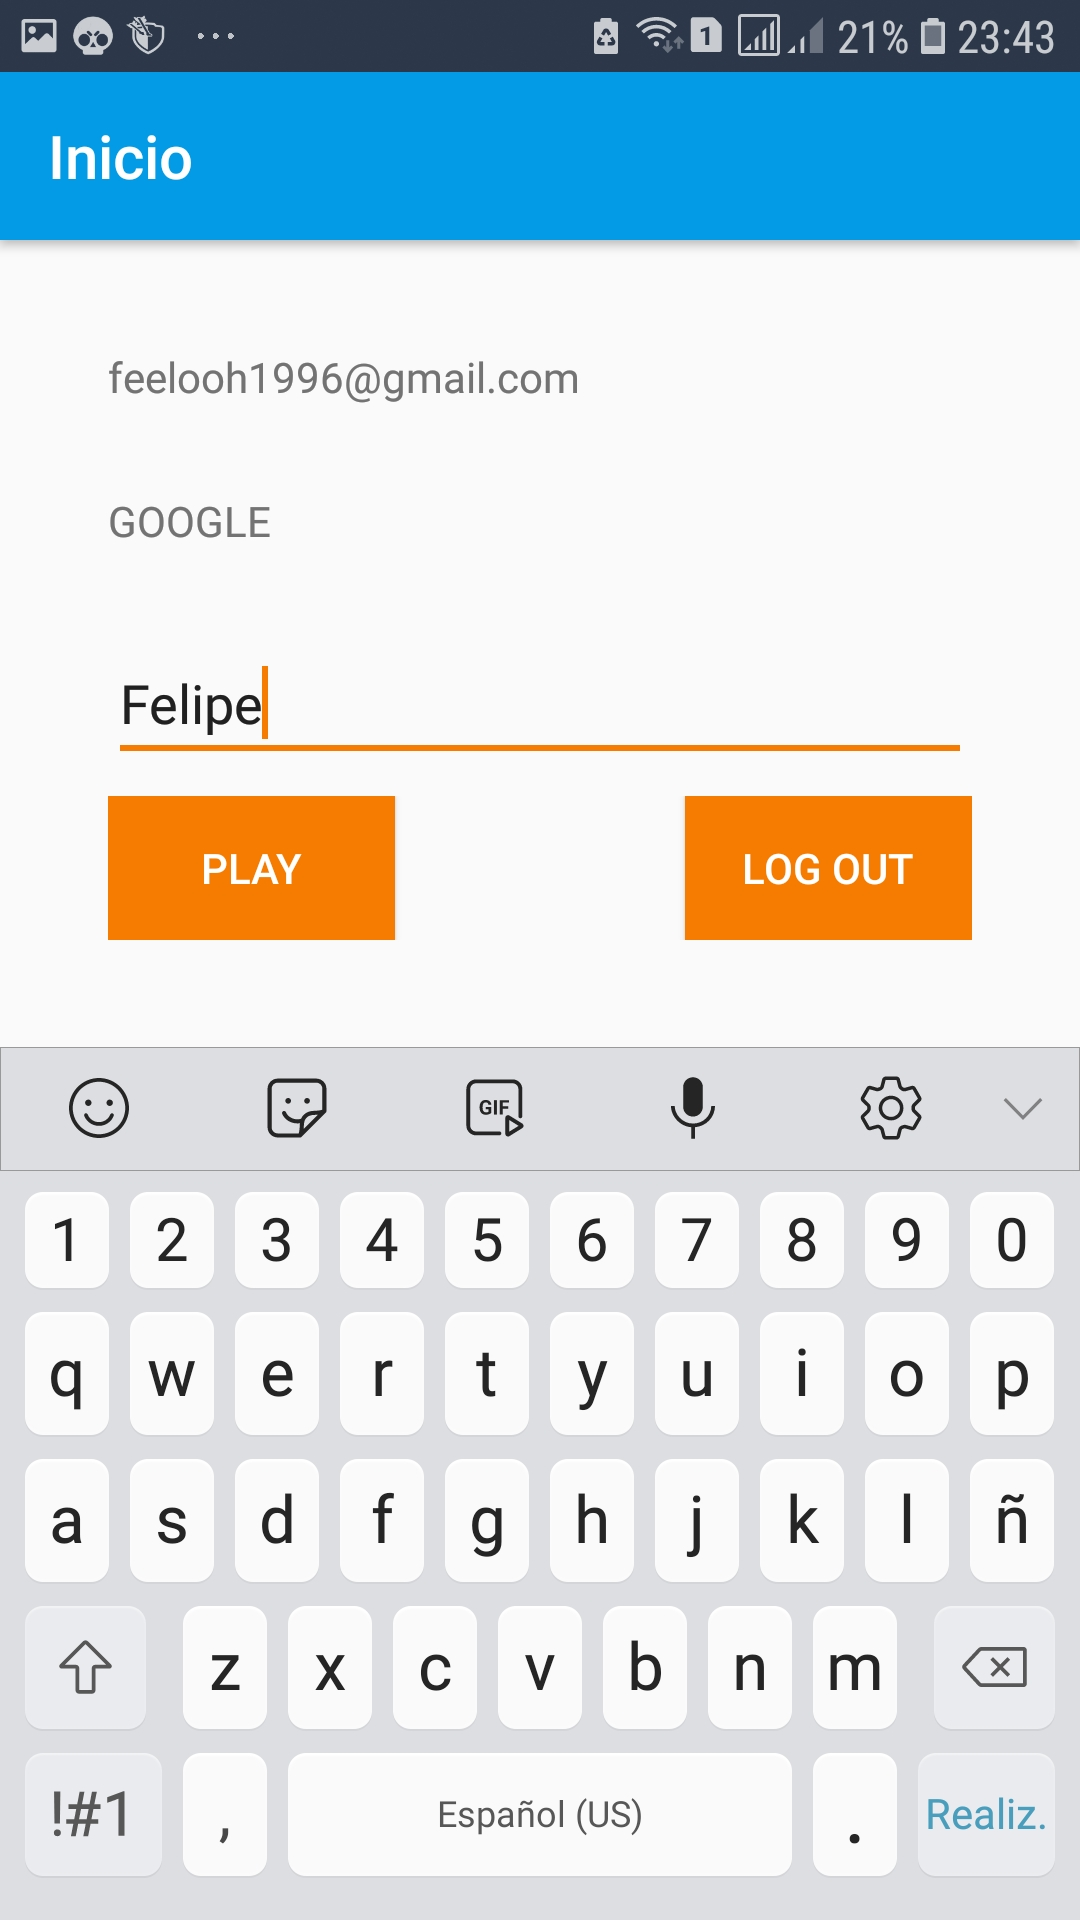
\includegraphics[width=5cm, height=8cm]{imgs/Screenshot3.jpg}}
 	\caption{Screenshot 1, 2 y 3}
\end{figure}
\begin{figure}[H]
	\centering
	\subfloat[Screenshot de la app N°04]
	{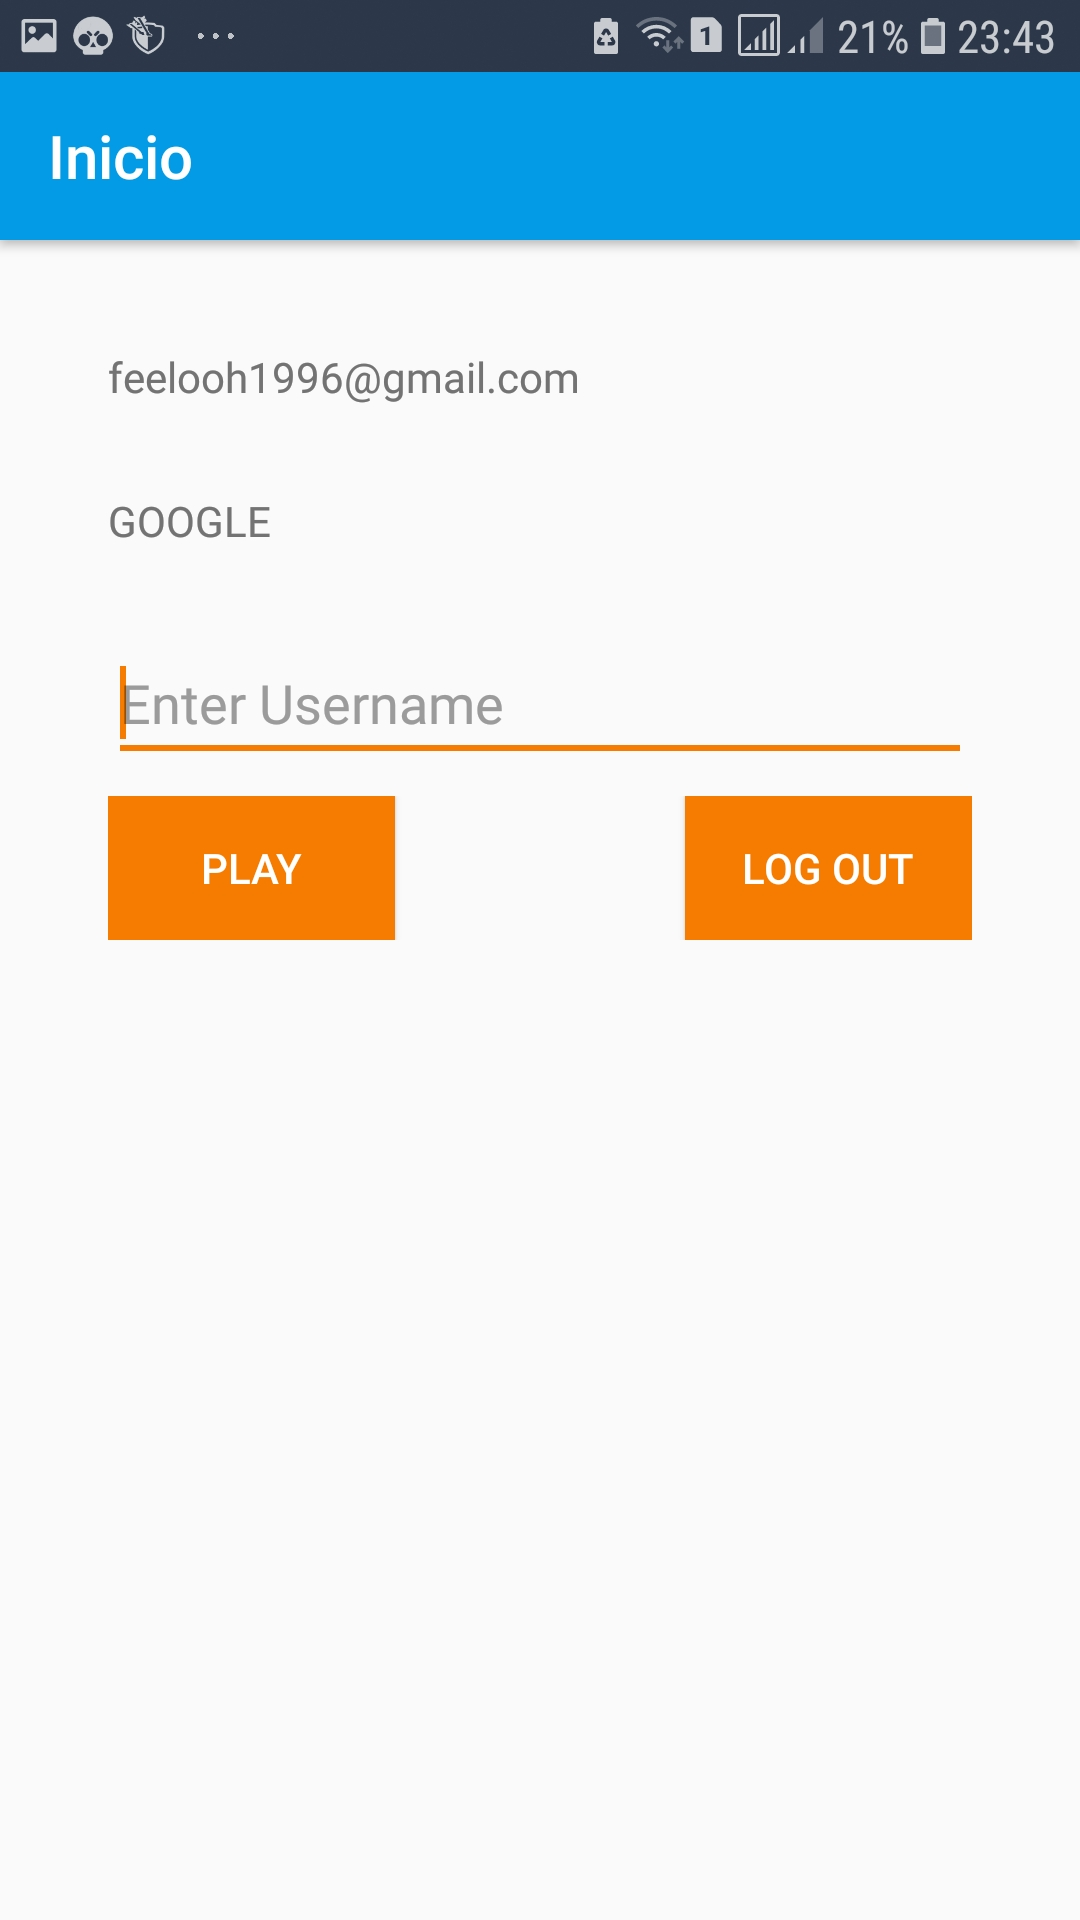
\includegraphics[width=5cm, height=8cm]{imgs/Screenshot4.jpg}}
	\subfloat[Screenshot de la app N°5]
	{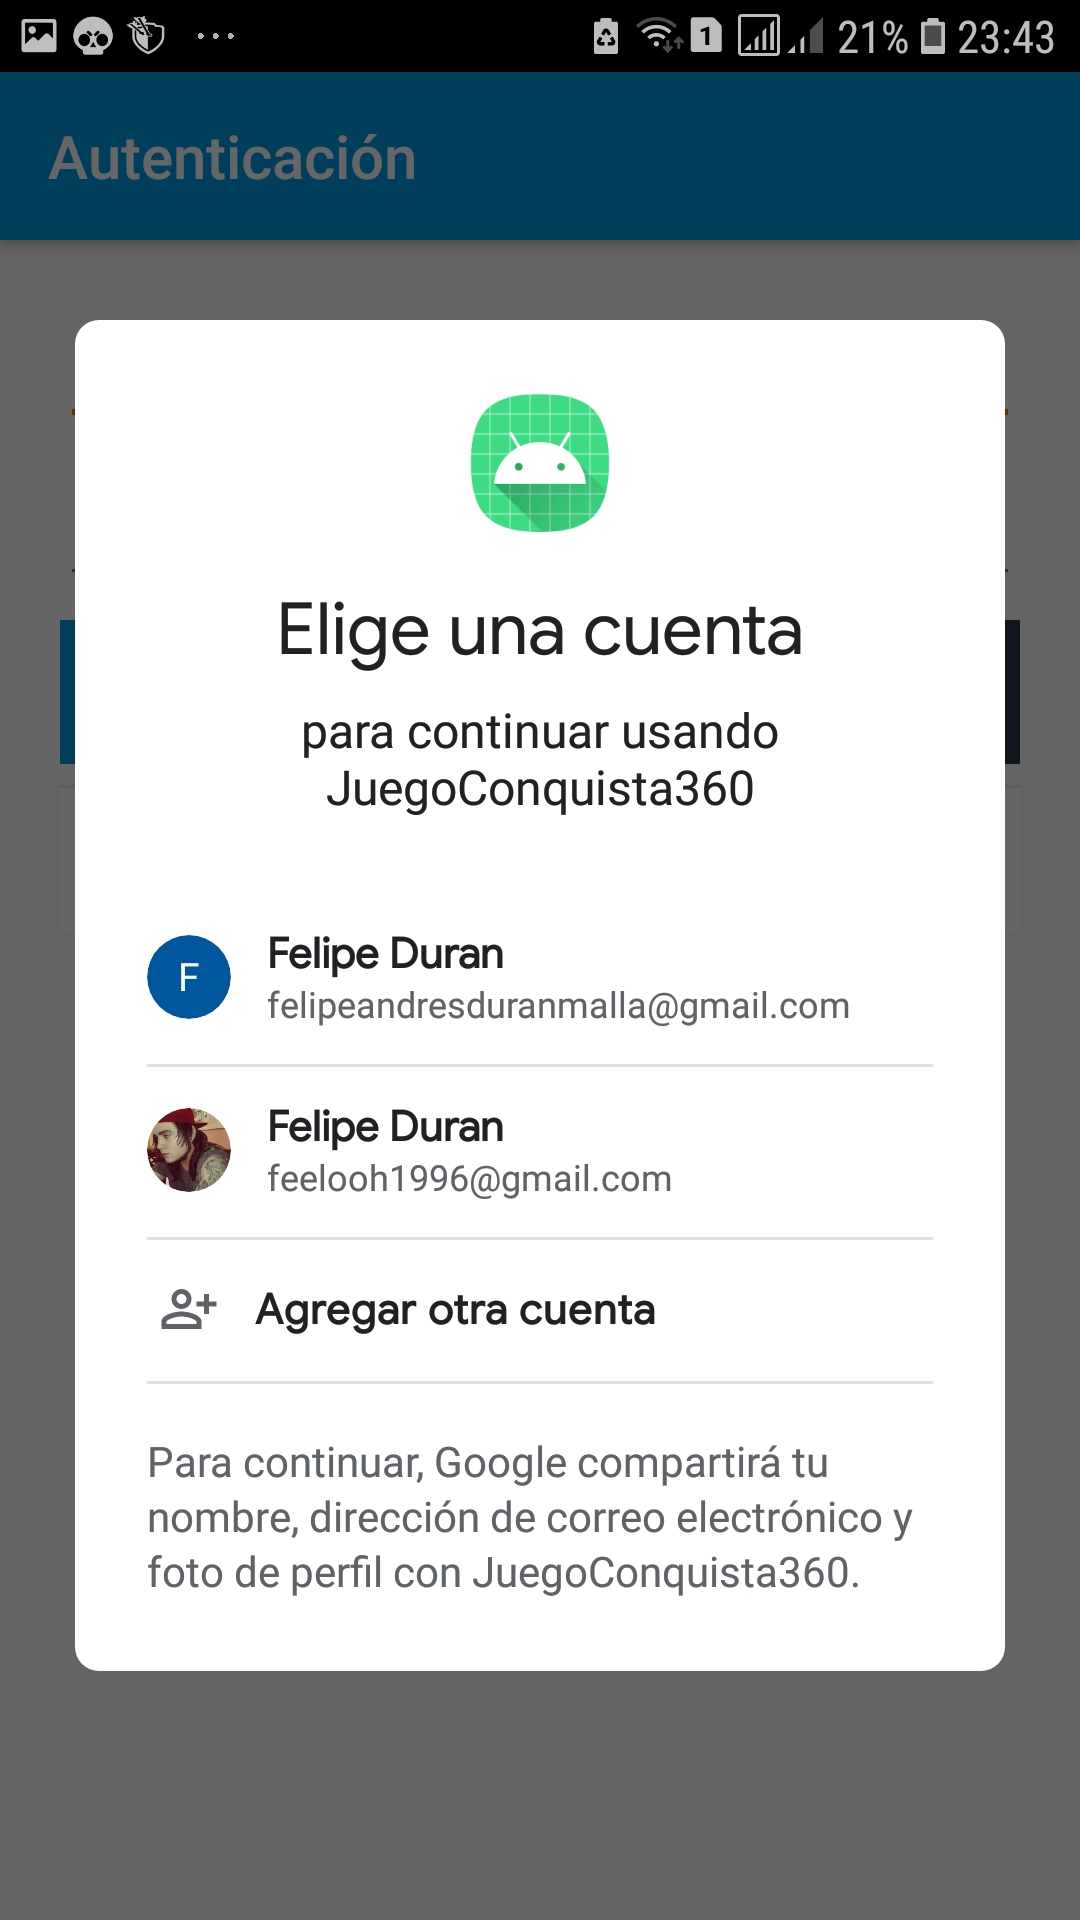
\includegraphics[width=5cm, height=8cm]{imgs/Screenshot5.jpg}}
	\subfloat[Screenshot de la app N°6]
	{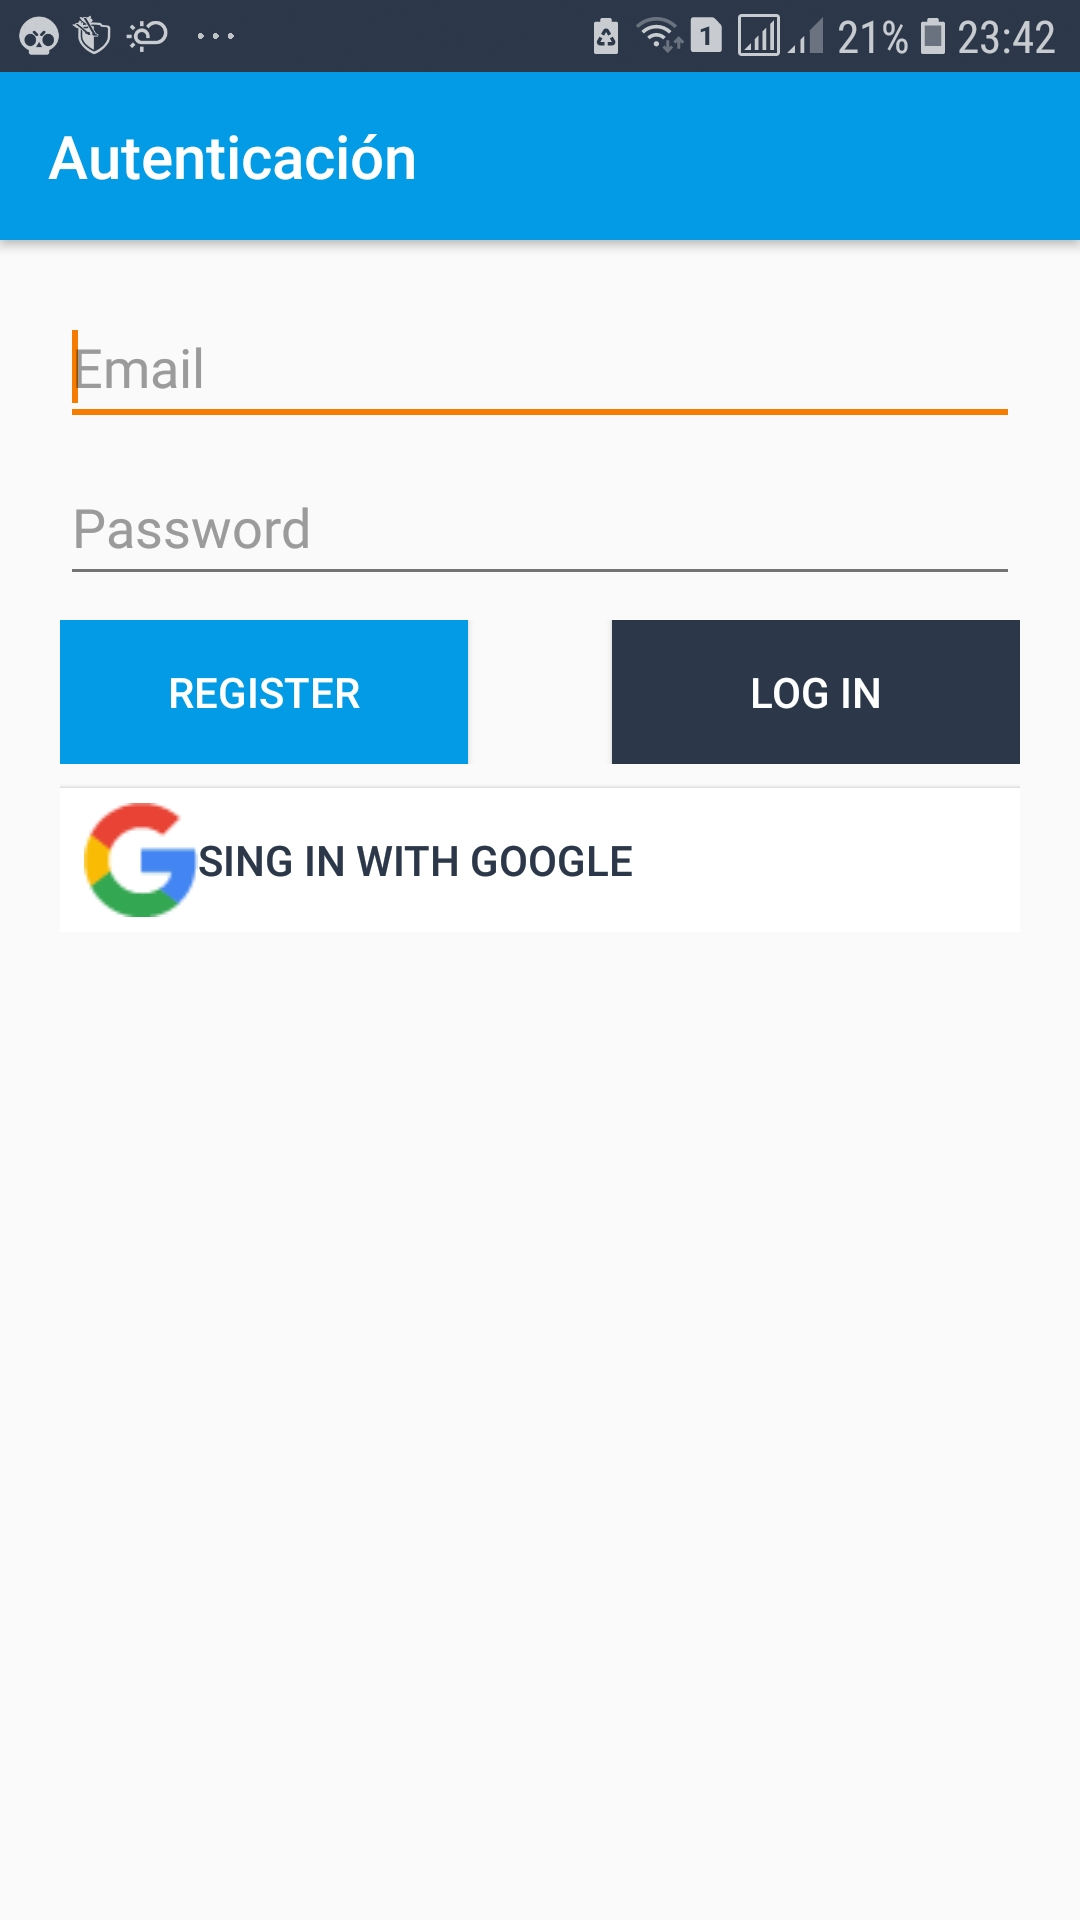
\includegraphics[width=5cm, height=8cm]{imgs/Screenshot6.jpg}}
 	\caption{Screenshot 4, 5 y 6}
\end{figure}



%%%%%%%%%%% DISEÑO %%%%%%%%%%%%%
%%%% Latex no permite el uso de 3 subsection por lo que \paragraph fue modificado para que cumpla con las caracteristicas de una subsection

\newpage
\section{Diseño}
\subsection{Derivación del Modelo de Software}
\subsubsection{Modelo de software inicial}
Tomando como base el modelo de dominio, el modelo de diseño inicial modifica mayormente el orden de las clases para definir de forma más lineal su funcionamiento, sin perder la función cíclica que la aplicación ya contiene.
La aplicación comienza con la identificación del usuario que además entrega una forma de reconocerse ante la base de datos. Luego de ingresar el jugador debe seleccionar una de las salas encontradas en la clase Room, donde además funciona como una forma de esperar a otros posibles jugadores. Al entrar al juego se mantiene el orden cíclico del modelo de dominio donde se puede ver la imagen en 360 y las palabras entregadas para luego crear la historia. Finalmente se entrega una valoración para los otros jugadores de sus historias que culmina con la presentación del ganador de la ronda, es decir, el jugador con la mejor valoración, para lo cual se pase a otra ronda.
\begin{figure}[H]
	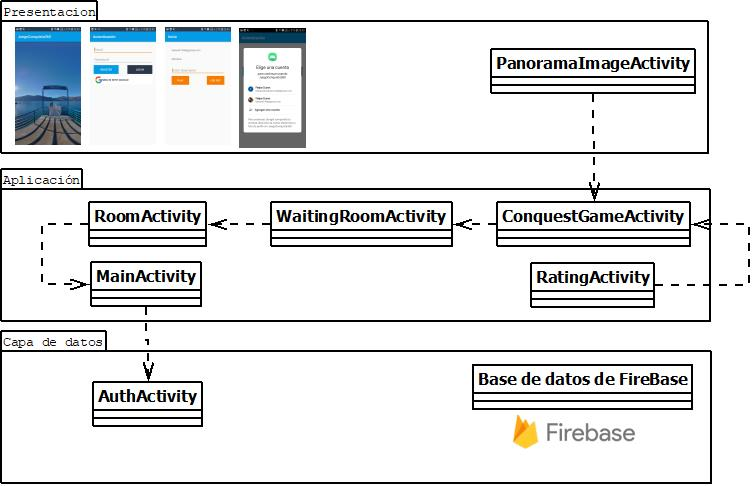
\includegraphics[width=16cm, height=20cm]{imgs/ModeloSoftwareInicial.jpg}
	\caption{Modelo de software inicial}
\end{figure}

\subsubsection{Diagramas de Clases}
A continuación se presenta el diagrama de clases utilisado en el desarrollo de nuestra aplicación, con el proposito de poder estudiar y analizar su estructura, funciones, atributos y composicion de manera mas gráfica y sencilla.

\begin{figure}[H]
	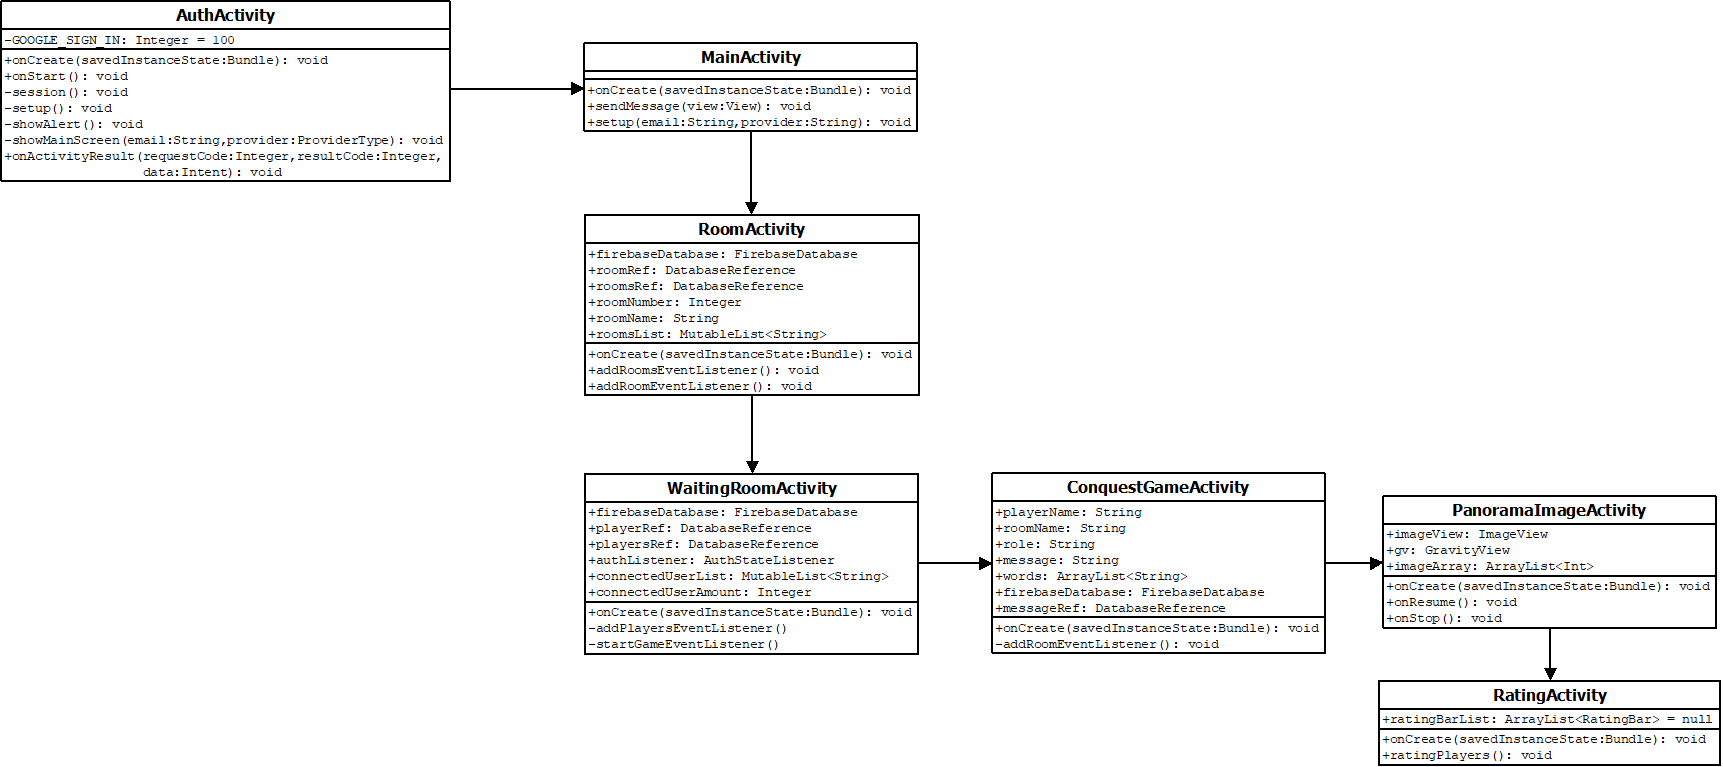
\includegraphics[width=16cm, height=9cm]{imgs/uml_isw.png}
	\caption{Diagrama de clases de diseño (UML)}
\end{figure}
\newpage
\subsubsection{Diagramas de Interacción}
Los diagramas de interaccion que se presentan a continuación grafican el recorrido de accion de los contratos presentados anteriormente en las tablas \ref{Contrato1}, \ref{Contrato2}, \ref{Contrato3}, \ref{Contrato4}, \ref{Contrato5} y \ref{Contrato6}.
\bigskip
\begin{enumerate}[1.]
	\item \textbf{Cargar Imagenes:}
El juego carga la imágenes una vez dentro de la partida, para así optimizar lo mejor posible el funcionamiento de la app, es por eso que, luego de ingresar a una partida en “RoomActivity”, el juego carga las imagenes en “ConquestGameActivity”.
	\begin{figure}[H]
		\centering
		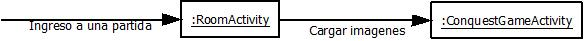
\includegraphics[scale=1]{imgs/Cargar Imagenes.jpeg}
		\caption{Diegrama de interacción: Cargar Imagenes}
	\end{figure}

	\item \textbf{Inicio de juego:}
El inicio de juego y todas sus verificaciones para el correcto funcionamiento ocurren dentro de la clase “MainActivity”, en esta clase, cuya función y tal como su nombre lo indica, hace de sala principal para redireccionar a las distintas instancias y demás clases.

	\begin{figure}[H]
		\centering
		\includegraphics[scale=1]{imgs/Inicio de juego.jpeg}
		\caption{Diegrama de interacción: Inicio de juego}
	\end{figure}

	\item \textbf{Inicio de Sesión:}
El inicio de sesión occure de dos formas dependiendo si la aplicación reconoce un usuario ingresado anteriormente. Si se entra por primera vez, es decir, no hay recolección de una sesión iniciada el usuario pasa a la clase de identificación donde debe ingresar sus datos o su cuenta de google para pasar a la clase “MainActivity”. En el caso de que ya se encuentre un usuario se pasa directamente a “MainActivity”.
	\begin{figure}[H]
		\centering
		\includegraphics[scale=1]{imgs/Inicio de Sesión.jpeg}
		\caption{Diegrama de interacción: Inicio de Sesión}
	\end{figure}

	\item \textbf{Mostrar Palabras:}
Luego de que todos los usuarios se encuentren en la sala, se da inicio a la partida, donde el primer paso es mostrarles las palabras que deben utilizar para crear la historia, esto se hace por medio de la clase “ConquestGameActivity” presentando el pool de palabras a los usuarios.
	\begin{figure}[H]
		\centering
		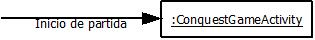
\includegraphics[scale=1]{imgs/Mostrar Palabras.jpeg}
		\caption{Diegrama de interacción: Mostrar Palabras}
	\end{figure}

	\item \textbf{Presentacion de puntaje:}
Luego de ingresar y ver las historias entregadas por todos los usuarios se pasa a la clase “RatingActivity”, donde todos ponen una nota a las historias creadas. Luego de que la aplicación se asegure de que todos los votos han sido ingresados como feedback, se vuelve a la clase de “ConquestGameActvity” donde se da inicio a la siguiente partida.
	\begin{figure}[H]
		\centering
		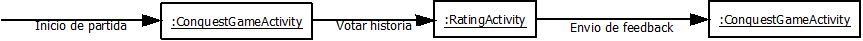
\includegraphics[scale=0.8]{imgs/Presentacion de puntaje.jpeg}
		\caption{Diegrama de interacción: Presentacion de puntaje}
	\end{figure}

	\item \textbf{Ver Imagen 360°:}
Una vez dentro de la partida la imagen del punto de conquista siempre estará visible para el jugador, y para mostrarla el juego debe acceder a la base de datos desde la clase”PanoramaImageActivity”, donde busca la imagen y la muestra al usuario.

	\begin{figure}[H]
		\centering
		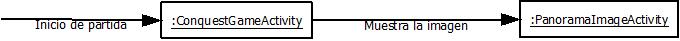
\includegraphics[scale=1]{imgs/Ver Imagen 360.jpeg}
		\caption{Diegrama de interacción: Ver Imagen 360°}
	\end{figure}
\end{enumerate}
\subsubsection{Diagramas de Estados}
Los diagramas de estado que se presentan en esta subseccion muestran el proceso de estados por los que pasa el programa segun sea el caso de uso en funcionamiento, mismos que se presentan en las tablas \ref{Contrato1}, \ref{Contrato2}, \ref{Contrato3}, \ref{Contrato4}, \ref{Contrato5} y \ref{Contrato6}.
\bigskip

\begin{figure}[H]
	\centering
	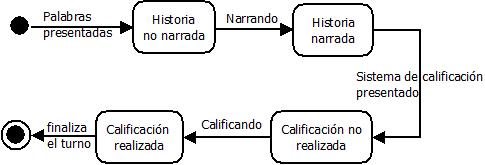
\includegraphics[scale=1]{imgs/DiagramaEstado1.png}
	\caption{Diegrama de estado: Jugar un turno}
\end{figure}

\begin{figure}[H]
	\centering
	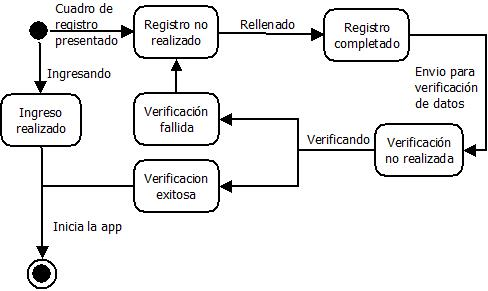
\includegraphics[scale=1]{imgs/DiagramaEstado2.png}
	\caption{Diegrama de estado: Iniciar sesión}
\end{figure}

\begin{figure}[H]
	\centering
	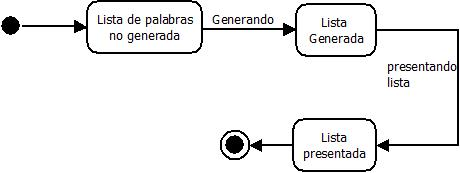
\includegraphics[scale=1]{imgs/DiagramaEstado3.png}
	\caption{Diegrama de estado: Gnerar lista de palabras}
\end{figure}

\begin{figure}[H]
	\centering
	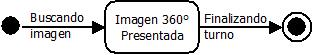
\includegraphics[scale=1]{imgs/DiagramaEstado4.png}
	\caption{Diegrama de estado: Mostrar Imagen 360°}
\end{figure}

\begin{figure}[H]
	\centering
	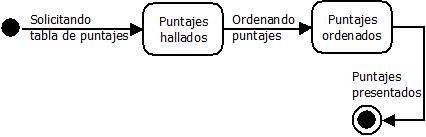
\includegraphics[scale=1]{imgs/DiagramaEstado5.png}
	\caption{Diegrama de estado: Mostrar tabla de puntaje}
\end{figure}

\begin{figure}[H]
	\centering
	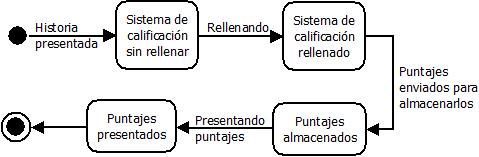
\includegraphics[scale=1]{imgs/DiagramaEstado6.png}
	\caption{Diegrama de estado: Puntuar jugador}
\end{figure}
\subsection{Refinamientos}
\subsubsection{Lugar de Refinamiento}
A pesar de no haberle dedicado mucho tiempo a esta sección en particular, nos hemos ido dando cuenta de ciertos puntos que requieren nuestra atención, por ejemplo, mejorar el diseño de la interfaz y la comunicación de esta con el usuario, integrar mas opciones que permitan al usuario personalizar la aplicación (Cambiar idioma, vincluar con diversas redes sociales, etc.), entre algunas de las opciones que hemos barajado, tambien estamos analizando la posibilidad de incluir un mejor sistema de jugabilidad, dando pie con esto ultimo a la opcion de abarcar aun a mas público, generando para esto distintos niveles de dificultad para hacer la experiencia de juego mas entretenida he interesante.
\subsubsection{Para cada Lugar}
\paragraph{Refinamientos considerados}
Los refinamientos considerados fueron obtenidos mediante el desarrollo de la idea general y su proposito, mas no gracias a un proceso de iteración donde estudiemos mejoras al rendimiento del software.

Los refinamientos son los siguientes:
\begin{enumerate}[1.]
	\item \textbf{Cambiar Idioma:} Tenemos la idea de añadir una opcion que permita al usuario cambiar el idioma del juego, esto nos daria a su vez la opción de promocionar el juego en distintos paises para permitir que nuestra cultura, y región sea conocida a traves del juego, sin necesidad de hablar español.
	\item \textbf{Vincular con redes sociales:} Esta idea surge de la necesidad de poder llegar a una mayor cantidad de público.
	\item \textbf{Generar niveles de dificultad:} Con esta modificación el juego ya no solo seria mas variado, si no que tambien lo haria menos reiterativo (Mucho menos de lo que ya es), ademas le da la posibilidad a la app de adaptarse al nivel de lenguaje del usuario que usara la app.
\end{enumerate}
\paragraph{Selección y descripción de una opción}
\textbf{Generar niveles de dificultad:} Este refinamiento se planea aplicar por medio de programar en el sistema una opcion que, al momento de crear una sala de juego, se presentepara moderar y adecuar el nivel de dificultad que el usuario quiera, presentando con la opción, las palabras que se incluiran y la cantidad de estas que se presentaran para la realisación de la historia. Junto con esto se añaden tambien, mas palabras a la base de datos y una clasificación para reconocer que dificultad posee la palabra en cuestion, asi, a la hora de generar una lista de palaras, estas se busquen tomando en concideración la caracteristica antes señalada.

%%%%%%%%%%%%%% IMPLEMENTACION %%%%%%%%%%
\newpage
\section{Implantación}
\subsection{Código fuente completo (parcial)}
\begin{figure}[H]
	\centering
	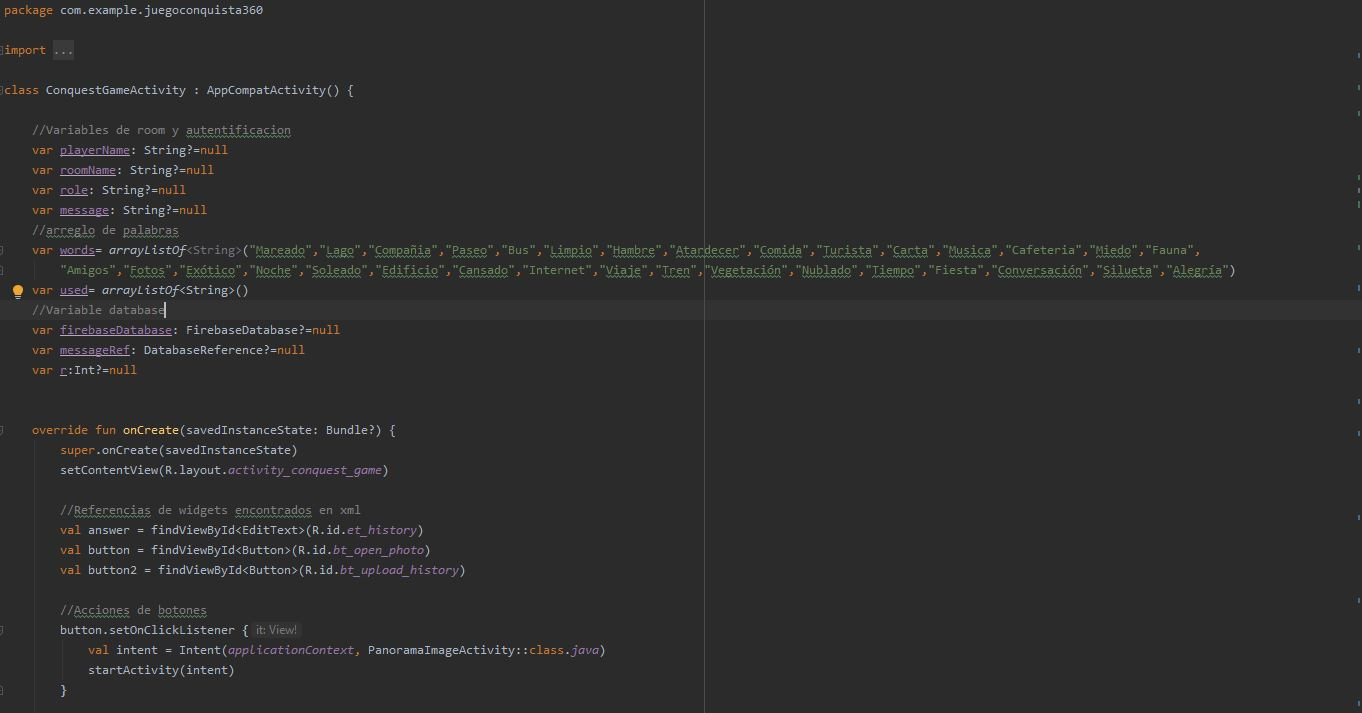
\includegraphics[scale=1]{imgs/SourceCode1.png}
	\caption{Codigo Clase ConquestGameActivity parte 1}
\end{figure}
\begin{figure}[H]
	\centering
	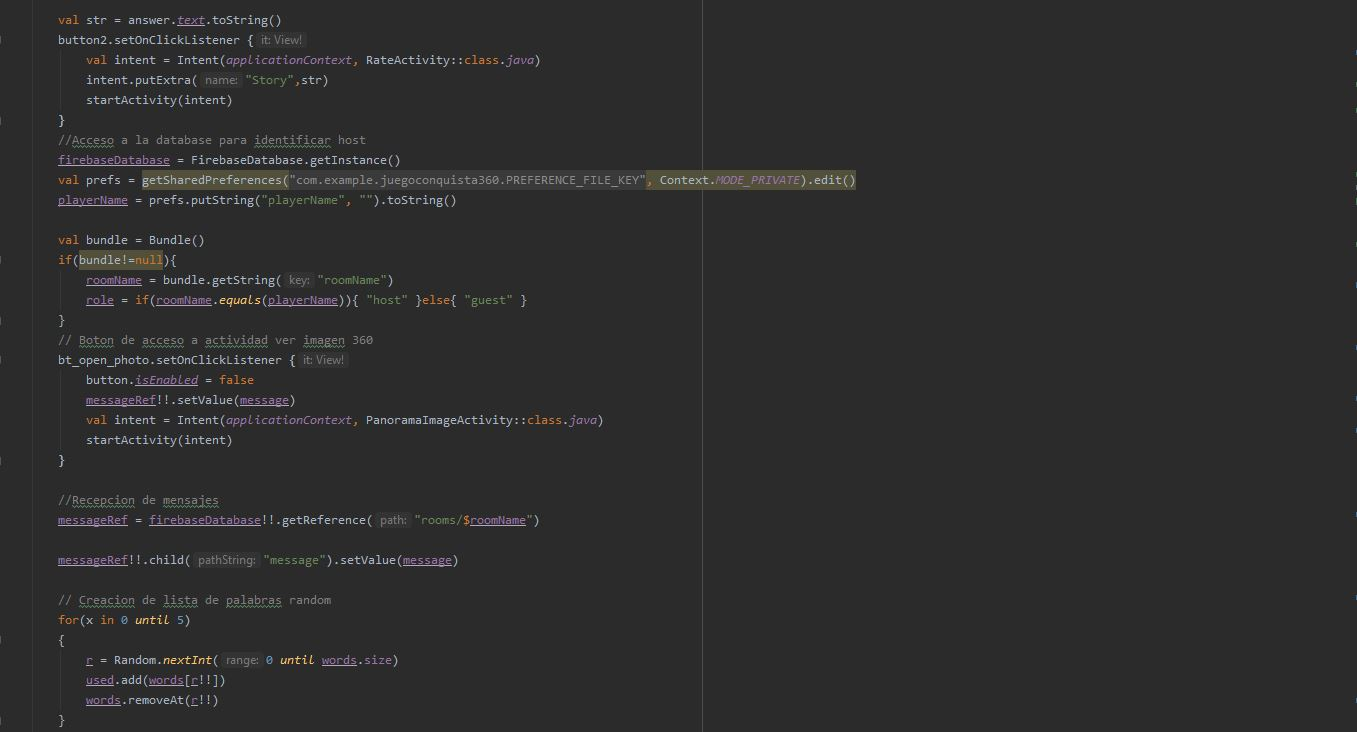
\includegraphics[scale=1]{imgs/SourceCode2.png}
	\caption{Codigo Clase ConquestGameActivity parte 2}
\end{figure}
\begin{figure}[H]
	\centering
	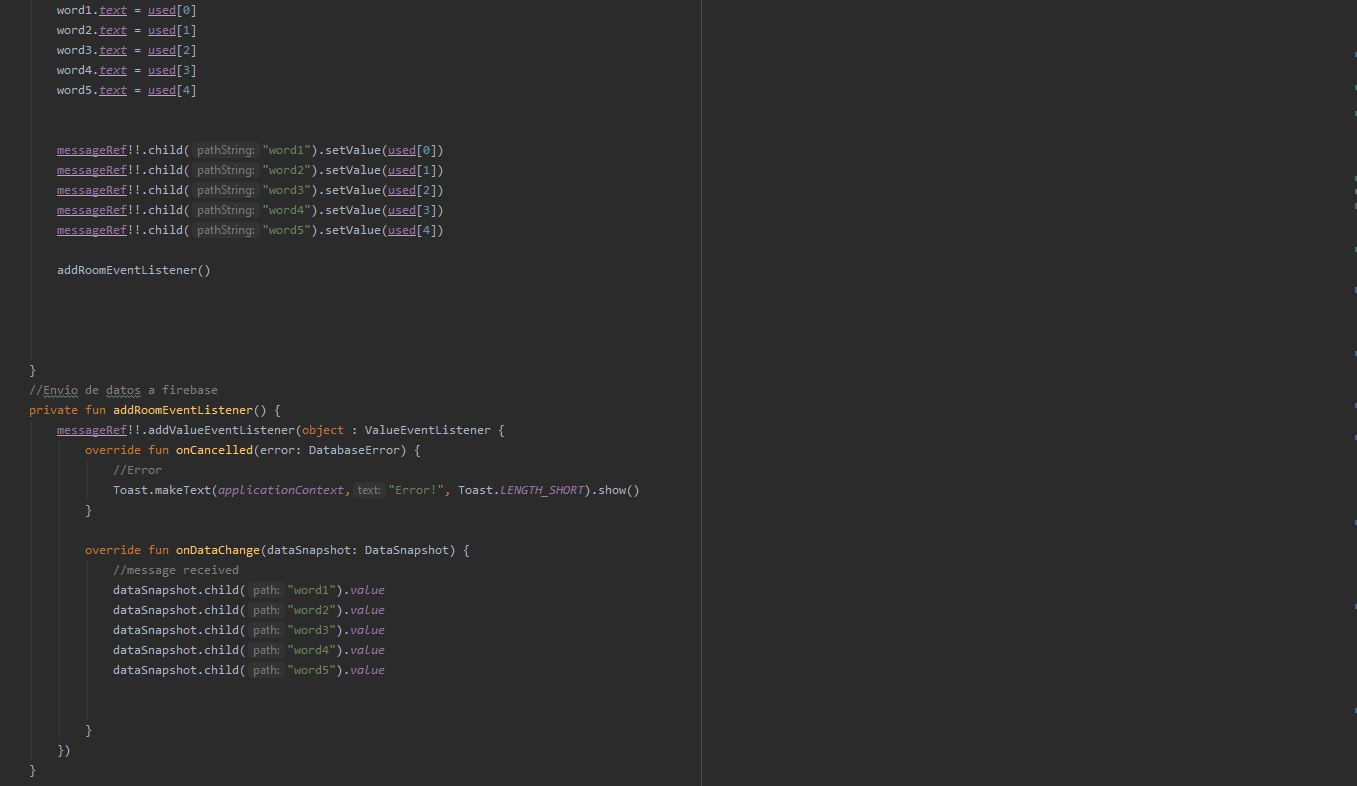
\includegraphics[scale=1]{imgs/SourceCode3.png}
	\caption{Codigo Clase ConquestGameActivity parte 3}
\end{figure}
\subsection{Modelo de implantación}
\subsection{Dependencias}

%%%%%%%%%%%%%%%% ANEXOS %%%%%%%%%%%%%%%%5
\newpage
\section{Anexos}
\subsection{Glosario}
\end{document}
